\documentclass[twoside]{article}

\usepackage{amsmath}
\usepackage{tikz} % graphics
\usepackage[sc]{mathpazo} % Use the Palatino font
\usepackage[T1]{fontenc} % Use 8-bit encoding that has 256 glyphs
\linespread{1.05} % Line spacing - Palatino needs more space between lines
\usepackage{microtype} % Slightly tweak font spacing for aesthetics

\usepackage[hmarginratio=1:1,top=32mm,columnsep=20pt]{geometry} % Document margins
\usepackage{multicol} % Used for the two-column layout of the document
\usepackage[hang, small,labelfont=bf,up,textfont=it,up]{caption} % Custom captions under/above floats in tables or figures
\usepackage{booktabs} % Horizontal rules in tables
\usepackage{float} % Required for tables and figures in the multi-column environment - they need to be placed in specific locations with the [H] (e.g. \begin{table}[H])
\usepackage{hyperref} % For hyperlinks in the PDF

\usepackage{lettrine} % The lettrine is the first enlarged letter at the beginning of the text
\usepackage{paralist} % Used for the compactitem environment which makes bullet points with less space between them

\usepackage{abstract} % Allows abstract customization
\renewcommand{\abstractnamefont}{\normalfont\bfseries} % Set the "Abstract" text to bold
\renewcommand{\abstracttextfont}{\normalfont\small\itshape} % Set the abstract itself to small italic text

\usepackage{titlesec} % Allows customization of titles
\renewcommand\thesection{\Roman{section}} % Roman numerals for the sections
\renewcommand\thesubsection{\Roman{subsection}} % Roman numerals for subsections
\titleformat{\section}[block]{\large\scshape\centering}{\thesection.}{1em}{} % Change the look of the section titles
\titleformat{\subsection}[block]{\large}{\thesubsection.}{1em}{} % Change the look of the section titles

\usepackage{fancyhdr} % Headers and footers
\pagestyle{fancy} % All pages have headers and footers
\fancyhead{} % Blank out the default header
\fancyfoot{} % Blank out the default footer
\fancyhead[C]{Vowel Classification $\bullet$ May 2015} % Custom header text
\fancyfoot[RO,LE]{\thepage} % Custom footer text


\title{\vspace{-15mm}\fontsize{24pt}{10pt}\selectfont\textbf{Support Vector Machines for SAE Vowel Phoneme Classification}} % Article title

\author{
\large
\textsc{Alan Zaffetti}\\[2mm]
\normalsize University of Massachusetts \\ 
\normalsize \href{mailto:azaffett@umass.edu}{azaffett@umass.edu}
\vspace{-5mm}
}
\date{}

\begin{document}

\maketitle

\begin{abstract}
In this study I use support vector machines to classify vowel phonemes from data.  Using the scikit-learn system, I train a model on vowel phoneme data covering twelve different standard American English vowel phonemes.  I will start by giving an introduction to SVMs as a model for multi-class classification.  I elaborate on my methods and relate them to similar studies.  I then present my results and calculate classification precision and recall per vowel.  I close with a discussion of the errors and how they are related to, and differ from those a human might make.
\end{abstract}

\begin{multicols}{2}

\tableofcontents

\section{Introduction}

\subsection{Phoneme Classification}

Phoneme classification is the task of decoding vowel identities given data on the frequencies of a voice graphed over time.

This graph data is comprised of what are known as formants which vary over time for each phoneme, exactly defining a sound, and in the human speech case, potentially sketch out a phoneme.

Some phoneme formants can form hard stops, and quick releases, some bending and changing over time. A plot showing frequency over time is known as a spectrogram plot.

The shape of these at different time periods can be extracted to fit feature vectors.  Its a corpus of these such feature vectors, the Hillenbrand vowel data, that I use for this project.

Vowels phonemes are found in the nucleus of the utterance.

\subsection{Classification Problem}

The ability to classify and recognize things in general is cental to human cognition.

The task is important enough to  motivate the design of systems which try to replicate this behavior.

The problem of vowel phoneme classification is dually tied, both to automated speech recognition systems, and to the cognitive machinery inside of us, specifically designed to processing auditory signals.

Beyond the engineer's motive, the question of whether a given model can reporduce the performace of human auditory machinery, can give insight into a possible configuartion of the machinery itself, how it might relate, and differ.

\subsection{Support Vector Machines}

A support vector machine is a linear binary classifier model.  It learns data which it represents in the form of feature vectors.  These feature vectors are projected to a space, and an optimization algorithm finds a linear seperation for the data into one of two classes usually called $\{+1,-1\}$.

A general support vector machine can be represented mathematically as
\begin{align}
u=\sum_i^N{y_i \alpha_i \boldsymbol{K}(\vec{x}_i, \vec{x}) - b}
\end{align}
where $u$ is the output of the SVM, a sum over all stored training examples $\vec{x}$ (vectors in the space), where $y_i\in\{+1,-1\}$ is the expected class for the $i^{th}$ training example, and $b$ is a threhold value.
$\boldsymbol{K}$ is what is known as the kernel function.

\subsubsection{As a Multiclass Model}

Since SVCs are in their nature binary classifiers, we must find ways to adapt the model for multiple classes, as required by the vowel case.  Luckily, methods exist for getting multiclass classifiers from regular linear SVCs.

\textbf{One-v.-one} method creates a classifier for each class $c$ against a class $c^\prime$ for each $c\neq c^\prime$.  This involves the creation of $O(n^2)$ classifiers each designed to compare two different classes, in our case two differnt vowel types. 

\textbf{One-v.-many} method creates $O(n)$ classifiers, each testing a vowel class $c$ against its complement $\bar{c}$ (every other vowel). Although this requires the creation of less classifiers in total, it can be less accurate over all.

Sci-learn SVC package implements the one-v.-one method, and I chose to go with this because, although its less space- and memory- efficient it might lead to better results \cite{smo}.

\subsubsection{The Kernel Method}

A Kernel function $\boldsymbol{K}$ is a vector function $f:X\times X\rightarrow\Re$ which determines the similarity between training examples.

In a broad sense, kernel function use avoids the explicit mapping that is needed to get linear learning algorithms to learn a nonlinear function or decision boundary.

Many kernel functions exist, but some work better than others for this task.  I found the best kernel functions for vowel classification to be the linear basis function
\begin{align}
f=\langle x,x^\prime \rangle
\end{align}
 and the polynomial basis function
 \begin{align}
f=(\gamma \langle x,x^\prime \rangle)^d \cdot d
\end{align}
where $d$ is a degree parameter in my model.

\section{Methods}

\subsection{Hillenbrand Vowel Data}

One of the two major components for this project was the Hillenbrand vowel corpus \cite{Hillenbrand} which contains a large amount of vowel data.

The corpus comes in two sizes, one with more detail than the other.  The smaller one contains rough measurements at 30\% vowel duration incremements, while the full data uses 10\% increments.

The corpus features vowels placed inbetween a $h\cdots d$ word frame, with nearly 150 speakers, and 12 total vowels.

Because of the efficiency of the kernel method for training SVMs, the model excels at high-dimensional data.  So, there's really an advantage to using the full dataset as will be discussed in the next section.

\subsection{Data Management}

I loaded the data from the \emph{.dat} file using regular expressions.  When testing the data, I used 5-part cross-validation and analysed the results as a confusion matrix, which I present in the next section.

If your looking at the source code (in \texttt{data.py}) you may notice the boolean toggle flags at the top of the code.  These allow you to switch between using the full and coarse the Hillenbrand dataset and which vowelset you're using (all 12 or just the 3).

\subsection{SVM Model}

The scikit-learn \cite{sklearn} system provided me with my SVM model as well as a wealth of easy-to-use statistical methods.  The SVM was parameterized and quite easy to change.

The polynomial basis kernel with a degree of 6 was the setting I found fit best, but other sources recommend a degree of 10 \cite{smo}.

Take a look at the \textit{svc.py} source file to see just how easy training a classifier is.

\section{Results}

\subsection{Classification Accuracy}

\subsubsection{Simplified 3 Vowels}

I achieved ceiling-level classification accuracy for \textbf{i}, \textbf{a}, and \textbf{u} (front, open, back) using both the linear and poly kernels 99\% (std=$\pm.02$), and 100\%, accuracies, respectively, using the full dataset.

Throughout, I kept the cross-validation at 5-parts and allocated 50\% of the data for training and testing.

There are no errors in either confusion matrix for the simplified vowelset:

\begin{align}
\begin{pmatrix}
	\textbf{i} & \textbf{a} & \textbf{u}
\end{pmatrix} \times
\begin{pmatrix}
	\textbf{i} \\
	\textbf{a} \\
	\textbf{u} \\
\end{pmatrix} =
\begin{pmatrix}
69 & 0  & 0   \\
 0 & 71 & 0   \\
 0 & 0  & 69  \\
\end{pmatrix}
\end{align}

This provides strong evidence that the SVM model is successful, at least as far as the simplest possible 3-class example takes it.

\subsubsection{All 12 Vowels}

The test on the full set of vowels proved more erroneous. I achieved classification accuracy for all vowels using both the linear and poly kernels 90\% (std=$\pm.06$), and 92\% (std=$\pm.05$), accuracies, respectively, on the full dataset.

Refering to the confusing matrix in \textbf{Figure 1}, it's interesting to see which vowels are confused the most.

\textit{ah} and \textit{aw} are confused the most (12/10).

\textit{ei} and \textit{iy} are mixed up at rates of (9/8).

And other vowels were mixed up $\leq3$ times in the test data.

I find these errors to be interesting because one can see by looking at $\textbf{Figures 1,2}$ that these vowels come close to one another in both the formant graph, and the vowel charts.

\section{Conclusion}

I used Python, NLTK \cite{nltk}, the Hillenbrand vowel corpus, and the sk-learn toolkit, to train support vector classifiers on the vowel phoneme classification problem.

I produced a program capable of classifying a sound based on measured formant frequency values into one of 12 vowel classes.  The program achieved over 90\% accuracy in the hard case.

An interesting discussion surrounds how the Human auditory system might function similarly to the models produced in this project.

Perhaps, cognitive machinery, like SVMs, are embedded in the nueral networks of every human, working at the symbolic level to understand the various frequencies of sounds they receive.

However, I cannot show just because the classifier errors are human-like, that the underlying systems share any simularities beyond this.

In any case, I have shown that SVMs are successful at vowel classification, and even compete with humans in determining vowel identity.

\begin{thebibliography}{9}

% http://ieeexplore.ieee.org/stamp/stamp.jsp?arnumber=4530027
\bibitem{smo}
  Boujelbene, Mezghani, Ellouze,
  \emph{Vowel Phoneme Classification Using SMO Algorithm for Training Support Vector Machines},
  2008.

% http://scikit-learn.org/
\bibitem{sklearn}
  Pedregosa, F. and Varoquaux, G. and Gramfort, A. and Michel, V. and Thirion, B. and Grisel, O. and Blondel, M. and Prettenhofer, P. and Weiss, R. and Dubourg, V. and Vanderplas, J. and Passos, A. and Cournapeau, D. and Brucher, M. and Perrot, M. and Duchesnay, E.,
  \emph{Scikit-learn: Machine Learning in {P}ython},
  Journal of Machine Learning Research,
  Volume 12, pp. 2825--2830, 2011.
  
% nltk.org
\bibitem{nltk}
  Bird, Steven, Edward Loper and Ewan Klein,
  \emph{Natural Language Processing with Python},
  O'Reilly Media Inc., 2009.
  
% homepages.wmich.edu/~hillenbr/
\bibitem{Hillenbrand}
	Hillenbrand, James,
	\emph{Vowel Data},
	Web, 1995.

\end{thebibliography}

\end{multicols}

\setcounter{MaxMatrixCols}{12}
\begin{figure}
\caption {Confusion matrix for all vowel data for the polynomial basis kernel on the full set of vowel classes.}
\centering
$\begin{pmatrix}
ae \\
ah \\
aw \\
eh \\
ei \\
er \\
ih \\
iy \\
oa \\
oo \\
uh \\
uw
\end{pmatrix} \times \cdots  =
\begin{pmatrix}
64 & 0 & 0 & 2 & 0 & 0 & 0&  0&  0&  0&  0&  0 \\
 3 &54 &10 & 0 & 0 & 1 & 0&  0&  0&  0&  0&  0 \\
 0 &12 &55 & 0 & 0 & 0 & 0&  0&  0&  0&  1&  0 \\
 8 & 0 & 0 &71 & 0 & 0 & 1&  0&  0&  0&  0&  0 \\
 0 & 0 & 0 & 0 &62 & 1 & 0&  8&  0&  0&  0&  0 \\
 0 & 0 & 0 & 2 & 0 &61 & 0&  0&  0&  0&  0&  0 \\
 0 & 0 & 0 & 1 & 0 & 0 &61&  0&  0&  0&  0&  1 \\
 0 & 0 & 0 & 0 & 9 & 0 & 0& 66&  0&  0&  0&  0 \\
 0 & 0 & 1 & 0 & 0 & 0 & 0&  0& 67&  0&  0&  3 \\
 0 & 0 & 0 & 1 & 0 & 0 & 0&  0&  0& 59&  3&  3 \\
 0 & 3 & 2 & 0 & 0 & 0 & 0&  0&  0&  0& 64&  0 \\
 0 & 0 & 1 & 0 & 0 & 0 & 1&  0&  1&  1 & 0& 70
\end{pmatrix}$
\end{figure}

\begin{figure}
\caption{A standard vowel chart.}
\centering
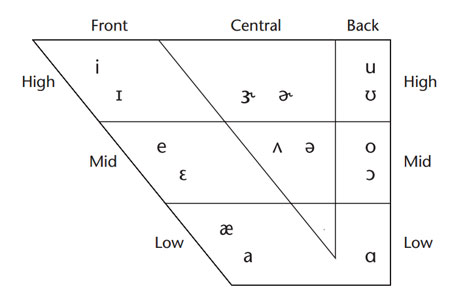
\includegraphics[scale=.5]{../figures/vowel-chart.jpg}
\end{figure}

\begin{figure}
\caption{A plot of $F_1$ and $F_2$ for vowels showing the overlap in some classes.}
\centering
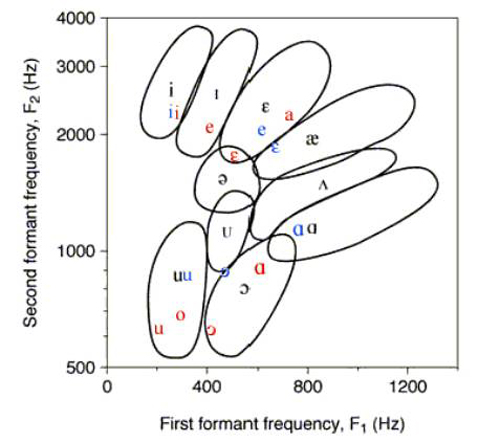
\includegraphics[scale=.5]{../figures/vowelchart.jpg}
\end{figure}

\end{document}